\documentclass[11pt]{article}
%\usepackage[paperwidth=8.5in, paperheight=11in]{geometry}
\usepackage[a5paper, landscape]{geometry}
\usepackage{tikz}

\usepackage{../tjimo}
\usepackage{graphicx}
%\usepackage[pdftex]{graphicx}

\begin{comment}
\def\answer{\comment}
\def\solution{\comment}
\def\solutionone{\comment}
\def\solutiontwo{\comment}
\end{comment}

\newcommand{\sevenpoints}{Time limit: 40 minutes.}
\newcommand{\righthead}{\fdbox{Round}{Guts}}

\DeclareMathOperator{\lcm}{lcm}

\begin{document}

\section*{Set 1}
\begin{problem}
What is $1 + 2 + 3 + 4 + \dots + 100$?
\end{problem}

\begin{answer}
5050
\end{answer}

\begin{solution}
Note that $100+1=99+2=98+3=\cdots=51+50=101$. Since there are $\frac{100}{2}=50$ of these pairs, we see that the sum is $50(101)=\boxed{5050}$.
\end{solution}

\begin{problem}
If an equilateral triangle has an area of $9\sqrt{3}$, what is the perimeter of the triangle?
\end{problem}

\begin{answer}
18
\end{answer}

\begin{solution}
The area of an equilateral triangle is $\dfrac{s^2\sqrt{3}}{4}$, where $s$ is the side length of the equilateral triangle. Equating this expression with $9\sqrt{3}$ gives us $s=6$, or a perimeter of $\boxed{18}$.
\end{solution}

\begin{problem}
Miranda is picking out skirts and crop tops to wear. If she has 5 skirts and 7 crop tops, how many outfits can she make?
\end{problem}

\begin{answer}
35
\end{answer}

\begin{solution}
Note that for every skirt, Miranda can wear any of the seven crop tops. This gives us a total of $5 \cdot 7 = \boxed{35}$ outfits. 
\end{solution}

\begin{problem}
What is the least common multiple of 6 and 4?
\end{problem}

\begin{answer}
12
\end{answer}

\begin{solution}
Since $6=2\cdot 3$ and $4=2^2$, the LCM is $2^2 \cdot 3=\boxed{12}$.
\end{solution}

\newpage
\section*{Set 2}
\begin{problem}
Gibbons drinks $\frac{1}{3}$ of the water in a bottle, and Ogden drinks $\frac{1}{4}$ of the remaining water. If there are 8mL of water left, how much water was there to begin with?
\end{problem}

\begin{answer}
16
\end{answer}

\begin{solution}
Gibbons drinks $\frac{1}{3}$ of the water, and Ogden drinks $\frac{2}{3} \cdot \frac{1}{4} = \frac{1}{6}$ of the water, leaving $1-\frac{1}{3} - \frac{1}{6} = \frac{1}{2}$ of the water remaining. Since $\frac{1}{2}$ of the water is 8 mL, there must have been $\boxed{16}$ mL of water to start with.
\end{solution}

\begin{problem}
I am drawing marbles out of a bag. If there are 3 red marbles and 5 blue marbles, what is the probability that the second marble I draw is red?
\end{problem}

\begin{answer}
$\frac{3}{8}$
\end{answer}

\begin{solution}
Note that the probability that the second marble is red is equal to the probabillity that the first marble is red. Thus, the answer is $\frac{3}{3+5} = \boxed{\frac{3}{8}}$.
\end{solution}

\begin{problem}
How many factors does 27 have?
\end{problem}

\begin{answer}
4
\end{answer}

\begin{solution}
$27 = 3^3$, so the only factors are 1, 3, 9, and 17, giving us a total of $\boxed{4}$ factors.
\end{solution}

\begin{problem}
If the radius of the larger circle is $6$, and all the smaller circles are the same size, what is the side length of the hexagon?
    \begin{center}
        \begin{tikzpicture}[thick, scale=0.6]
            \draw (0, 0) circle (3cm);
            \draw (0, 0) circle (1cm);
            \draw (2, 0) circle (1cm);
            \draw (-2, 0) circle (1cm);
            \draw (1, 1.73205080757) circle (1cm);
            \draw (1, -1.73205080757) circle (1cm);
            \draw (-1, 1.73205080757) circle (1cm);
            \draw (-1, -1.73205080757) circle (1cm);
            \draw (2, 0) -- (1, 1.73205080757) -- (-1, 1.73205080757) -- (-2, 0) -- (-1, -1.73205080757) -- (1, -1.73205080757) -- cycle;
        \end{tikzpicture}
    \end{center}
\end{problem}

\begin{answer}
4
\end{answer}

\begin{solution}
Consider the following diagram. 
    \begin{center}
        \begin{tikzpicture}[thick, scale=0.6]
            \draw (0, 0) circle (3cm);
            \draw (0, 0) circle (1cm);
            \draw (2, 0) circle (1cm);
            \draw (-2, 0) circle (1cm);
            \draw (1, 1.73205080757) circle (1cm);
            \draw (1, -1.73205080757) circle (1cm);
            \draw (-1, 1.73205080757) circle (1cm);
            \draw (-1, -1.73205080757) circle (1cm);
            \draw (2, 0) -- (1, 1.73205080757) -- (-1, 1.73205080757) -- (-2, 0) -- (-1, -1.73205080757) -- (1, -1.73205080757) -- cycle;
            \draw[color = red] (0, 0) -- (2, 0);
            \draw[color = blue] (0, 0) -- (1.5, 2.59807621);
        \end{tikzpicture}
    \end{center}

Note that if we draw in the red segment (shown above), it is equal to the sidelength of the hexagon. Thus, it is equal to two times the radius of a smaller circle. Also note that the radius of a smaller circle is equal to $\frac{1}{3}$ of the radius of the larger circle (see the blue line for reference). Thus, the side length of the hexagon is equal to $2 \cdot \frac{1}{3}=\frac{2}{3}$ of the larger radius, or $\frac{2}{3} \cdot 6 = \boxed{4}$.

\end{solution}

\newpage
\section*{Set 3}
\begin{problem}
If $A+B=4$, $C+D=8$, and $A+C=7$, what is $B+D$?
\end{problem}

\begin{answer}
5
\end{answer}

\begin{solution}
Adding the first two equations yields $A+B+C+D=12$. Subtracting $A+C=7$ gives us $B+D=\boxed{5}$.
\end{solution}

\begin{problem}
There is a 40\% chance of rain on Saturday. If it rains on Saturday, there is a 60\% chance of rain on Sunday. Otherwise, there is a 30\% chance of rain on Sunday. What is the probability it rains on Sunday?
\end{problem}

\begin{answer}
0.42
\end{answer}

\begin{solution}
If it rains on Saturday, there is a probability of $0.4 \cdot 0.6 =  0.24$ that it will rain on Sunday. If it doesn't rain on Saturday, there is a probability of $0.6 \cdot 0.3 = 0.18$ that it will rain on Sunday. Adding these up yields our desired answer of $\boxed{0.42}$.
\end{solution}

\begin{problem}
How many ways can I seat Josh, Akshaj, Jeffery, Katherine, Michael, and Wendy at a circular table so that Wendy and Katherine are sitting next to each other?
\end{problem}

\begin{answer}
48
\end{answer}

\begin{solution}
Let us fix Wendy and Katherine in two adjacent seats. Then, there are $4!=24$ ways to arrange the other 4 people. However, Wendy and Katherine can switch seats, which gives us a total of $24 \cdot 2 = \boxed{48}$ ways.
\end{solution}

\begin{problem}
Let $ABCD$ and $EFGH$ be squares such that $E$ lies on $AB$, $F$ lies on $BC$, $G$ lies on $CD$, and $H$ lies on $AD$. If the area of $EFGH$ is $\frac{5}{9}$ of the area of $ABCD$ and $AE \geq BE$, what is $\frac{AE}{BE}$?
\end{problem}

\begin{answer}
2
\end{answer}

\begin{solution}
Consider the following diagram.
\begin{center}
    \begin{tikzpicture}
        \draw (0, 0) -- (3, 0) -- (3, 3) -- (0, 3) -- cycle;
        \draw (1, 0) -- (3, 1) -- (2, 3) -- (0, 2) -- cycle;
        \node at (0, 0)[below left] {A};
        \node at (0, 3)[above left] {B};
        \node at (3, 3)[above right] {C};
        \node at (3, 0)[below right] {D};
        \node at (0, 2)[left] {E};
        \node at (2, 3)[above] {F};
        \node at (3, 1)[right] {G};
        \node at (1, 0)[below] {H};
    \end{tikzpicture}
\end{center}
Note that if the area of $EFGH$ is $\frac{5}{9}$ of the area of $ABCD$, the area of each of the right triangles must be $\frac{1}{9}$ of the area of $ABCD$. Thus, $(AE)(AH) = \frac{2}{9}[ABCD]=\frac{2}{9}AB^2$, where $[ABCD]$ is the area of $ABCD$. Since we know that $AE + AH = AE + BE = AB$, we see that $AE=\frac{2}{3}AB$ once we solve the system of equations. Thus, $\frac{AE}{BE} = \boxed{2}$.
\end{solution}
\newpage
\section*{Set 4}
\begin{problem}
For an art project, Katherine is building a model of TJ. If the real auditorium is 30 feet wide but 2 inches on Katherine's model, how long in feet should the model gym be if the real gym is 75 feet long?
\end{problem}

\begin{answer}
$\frac{5}{12}$
\end{answer}

\begin{solution}
Using proportions, we see that $\frac{2}{30} = \frac{x}{75}$, where $x$ is the length of the gym of the model in inches. Solving for $x$ gives $x=5$ inches, which is equal to $\boxed{\frac{5}{12}}$ feet.
\end{solution}

\begin{problem}
How many ways can I split 7 nondistinguishable pieces of candy among 4 distinguishable people, assuming each person gets at least one?
\end{problem}

\begin{answer}
20
\end{answer}

\begin{solution}
Using the method of sticks and stones (or stars and bars), we see that there are ${{7-1} \choose {4-1}} = {6 \choose 3} = \boxed{20}$ ways to split the candy.
\end{solution}

\begin{problem}
Gideon is facing trial, but he only has 10 dollars. If Wainwright offers lawyers for 3 dollars and evidence for 2 dollars each, how many combinations of lawyers and evidence can Gideon buy, assuming that he needs to buy a lawyer and he does not need to spend all 10 dollars?
\end{problem}

\begin{answer}
8
\end{answer}

\begin{solution}
Since Gideon needs to buy a lawyer, the problem is equivalent to Gideon not having to buy a lawyer and having 7 dollars total. Note that he cannot buy three or more lawyers. If he buys two additional lawyers, he cannot buy any evidence. If he buys one additional lawyer, he can buy up to two pieces of evidence, giving three possibilities. If he buys no additional lawyers, he can buy up to three pieces of evidence, yielding four possibilities. Summing this up, we have a total of $1+3+4=\boxed{8}$ combinations.
\end{solution}

\begin{problem}
Katherine, Neeyanth, Wendy, and Ryan are arguing over who is a freshman and who is an upperclassman. Freshmen always lie, while upperclassmen always tell the truth. 
    
Neeyanth says: Ryan is a freshman.
    
Ryan says: Out of Neeyanth and I, exactly one of us is a freshman.

Wendy says: There are not more freshmen than upperclassmen.
    
Katherine says: At most three of us are freshman.
    
\noindent Who is a freshman (list everyone)?
\end{problem}

\begin{answer}
Neeyanth
\end{answer}

\begin{solution}
If Neeyanth is not a freshman, then Ryan is a freshman, which means that both Neeyanth and Ryan are either freshmen or upperclassmen. Since this is a contradiction, Neeyanth must be a freshman and Ryan must be an upperclassman. Since we know Ryan is an upperclassman, there are at most three freshmen, and Katherine must be an upperclassman. Now that we have established that both Katherine and Ryan are upperclassmen, Wendy's statement is true regardless of whether or not she is an upperclassman, making her an upperclassman as well. Thus, Neeyanth is the only freshman.
\end{solution}

\newpage
\section*{Set 5}
\begin{problem}
Given that the median of 7 not necessarily distinct integers in the set $\{1, 2, 3, \dots 15\}$ is 8 and the distinct mode is 9, what is the largest possible mean?
\end{problem}

\begin{answer}
$\frac{59}{7}$
\end{answer}

\begin{solution}
There must be an 8 since there are 7 integers, and at least 2 9's. To maximize the mean, we should use 
\end{solution}

\begin{problem}
 What is the smallest positive integer that gives a remainder of 1 when divided by 3, a remainder of 3 when divided by 5, and 5 when divided by 7?
\end{problem}

\begin{answer}
103
\end{answer}

\begin{solution}
We can write this as $x \equiv -2 (\pmod 3)$, $x \equiv -2 (\pmod 5)$, and $x \equiv -2 (\pmod 7)$. Thus, the smallest possible value of $x$ is $\lcm (3, 5, 7) - 2 = 105-2 = \boxed{103}$
\end{solution}

\begin{problem}
Consider point $P$ which lies outside of circle $\omega$. $A$ and $B$ lie on $\omega$, $C \neq A$ is the intersection of $AP$ and $\omega$, and $B\neq D$ is the intersection of $BP$ and $\omega$. If $AC=7$, $AP=9$, $BD=10$, and $BP < DP$ what is $BP$?
\end{problem}

\begin{answer}
8
\end{answer}

\begin{solution}
By Power of a Point, we have $(BP)(DP) = (AP)(CP) = (9)(9+7) = 144$. We also have $DP-BP = 10$. Solving the system of equations yields our desired answer of $BP=\boxed{8}$
\end{solution}

\begin{problem}
What is the probability that if I flip a coin 8 times in a row, I get heads at least 4 times?
\end{problem}

\begin{answer}
$\frac{163}{256}$
\end{answer}

\begin{solution}
The probability of getting 4 heads and 4 tails is equal to $\frac{8 \choose 4}{2^8} = \frac{70}{256} = \frac{35}{128}$. Note that the probability of getting more than 4 heads is equal to the probability of getting more than 4 tails, which is equal to the probability of getting less than 3 heads. Thus, the probability of getting at least 4 heads is $\dfrac{1+\frac{35}{128}}{2} = \boxed{\frac{163}{256}}$
\end{solution}

\newpage
\section*{Set 6}
\begin{problem}
If $\frac{1}{1^2} + \frac{1}{2^2} + \frac{1}{3^2} + \dots = \frac{\pi^2}{6}$, what is $\frac{1}{2^2} + \frac{1}{4^2} + \frac{1}{6^2} + \ldots$?
\end{problem}

\begin{answer}
$\frac{\pi^2}{24}$
\end{answer}

\begin{solution}
Note that $\frac{1}{2^2} + \frac{1}{4^2} + \frac{1}{6^2} + \ldots = \frac{1}{(2 \cdot 1)^2} + \frac{1}{(2 \cdot 2)^2} + \frac{1}{(2 \cdot 3)^2} + \dots = \frac{1}{4}\left(\frac{1}{1^2} + \frac{1}{2^2} + \frac{1}{3^2} + \dots\right) = \frac{1}{4} \cdot \frac{\pi^2}{6} = \boxed{\frac{\pi^2}{24}}$
\end{solution}

\begin{problem}
How many triangles are in the following figure?
    
    \begin{center}
        \begin{tikzpicture}
            \draw (0, 0) -- (3, 0) -- (3, 3) -- (0, 3) -- cycle;
            \draw (1, 0) -- (3, 1) -- (2, 3) -- (0, 2) -- cycle;
            \draw (0, 1) -- (1, 3) -- (3, 2) -- (2, 0) -- cycle;
        \end{tikzpicture}
    \end{center}
    
\end{problem}

\begin{answer}
28
\end{answer}

\begin{solution}
Consider the following diagram.
\begin{center}
        \begin{tikzpicture}
            \draw (0, 0) -- (3, 0) -- (3, 3) -- (0, 3) -- cycle;
            \draw (1, 0) -- (3, 1) -- (2, 3) -- (0, 2) -- cycle;
            \draw (0, 1) -- (1, 3) -- (3, 2) -- (2, 0) -- cycle;
            \draw[color=blue] (1, 0) -- (1.5, 0.24) -- (0.67, 0.67) -- cycle;
            \draw[color=red] (3, 0) -- (3, 2) -- (2, 0) -- cycle;
            \draw[color=purple] (2, 3) -- (1, 3) -- (1.5, 2.76) -- cycle;
            \draw[color=green] (0, 2) -- (0, 1) -- (0.67, 2.33) -- cycle;
        \end{tikzpicture}
    \end{center}
There are 8 blue triangles, 8 red triangles, 4 purple triangles, and 8 green triangles, giving us a total of $\boxed{28}$ triangles.

\end{solution}

\begin{problem}
When 2017 is multiplied by a single digit nonzero integer $x$, all the digits are perfect squares. What is $x$?
\end{problem}

\begin{answer}
7
\end{answer}

\begin{solution}
In order for all the digits to be perfect squares, they must be 0, 1, 4, or 9. Consider the last digit. If it is a 0, then $x$ must be 0, which does not work. If it is 1, $x$ must be 3, which gives 6051, which does not work. It if is $4$, $x$ must be 2, which gives 4034, which doesn't work either. Thus, it must end with a 9, and $2017\cdot7=14119$, which satisfies the conditions, so $x=\boxed{7}$.
\end{solution}

\begin{problem}
Let each letter represent a distinct digit. If $J=8$ and $A$ is even, what is the five digit number $MAGIC$?
\[
    \begin{tabular}{c c c c c c}
        & T & J & I & M & O \\
        + & & M & A & T & H \\
        \hline
        & M & A & G & I & C
    \end{tabular}
\]
\end{problem}

\begin{answer}
42976
\end{answer}

\begin{solution}
Build a table using all the possibilities. Note that since $M$ and $T$ are distinct, $M=T+1$. Also, note that for each $T$, there are two possibilities for $I$ (if $O+H \geq 10$ and if $O+H < 9$).
\begin{center}
    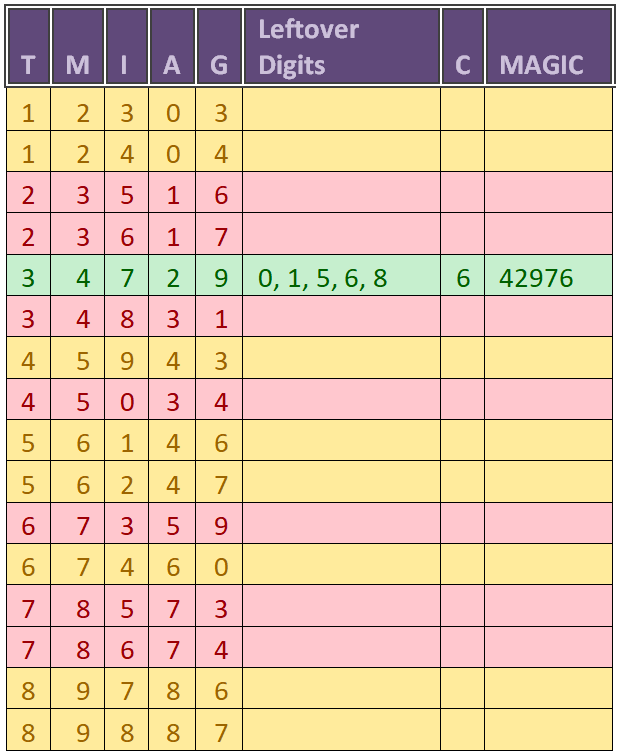
\includegraphics[scale=0.5]{guts_table}
\end{center}
Note that $A$ and $G$ are interdependent. $I+A=G$, or $I+A+1=G$ (depending on $M$ and $T$), and $J+M=A$ or $J+M+1=A$, depending on $I$ and $A$. We can find a distinct pair of $G$ for each triple of $(M, T, I)$. Everything in red does not have an even $A$, and everything in yellow does now have distinct digits. The remaining option is in green, with the only possibilities for $O$ and $H$ are 1 and 5, with $C$ being 6. Thus,  $MAGIC=\boxed{42976}$.
\end{solution}

\newpage
\section*{Set 7}
\begin{problem}
What is $\frac{1}{1\cdot2}+\frac{1}{2\cdot3} + \frac{1}{3*4} + \dots + \frac{1}{29\cdot30}$?
\end{problem}

\begin{answer}
$\frac{29}{30}$
\end{answer}

\begin{solution}
Note that $\frac{1}{n(n+1} = \frac{1}{n} - \frac{1}{n+1}$. Thus, the expression evaluates to $\frac{1}{1} - \frac{1}{2} + \frac{1}{2} - \frac{1}{3} + ... - \frac{1}{29} + \frac{1}{29} - \frac{1}{30} = 1-\frac{1}{30} = \boxed{\frac{29}{30}}$
\end{solution}

\begin{problem}
Allen the alien lives on Lelan. All 52 Lelans start the day by drawing a card without replacement from a single deck of 52 cards. If they get an ace, then they get the day off, and if they get a face card, they get the afternoon off. Allen forms a group with 2 other aliens so that if any of them get time off, they secretly swap cards so that Allen gets time off. What is the probability that Allen will get time off?
\end{problem}

\begin{answer}

\end{answer}

\begin{solution}
In order for someone other than Allen to get time off, at least one of the aliens must draw cards with time off. We will solve this by commplementary counting. In order for Allen to not get time off, no one can draw a card that gives time off. There are 4 aces and 12 face cards, so there are 16 cards which lead to time off. The probability that Allen does not get time off is $\dfrac{36}{52}\cdot \dfrac{35}{51} \cdot \dfrac{34}{50} = \dfrac{21}{65}$. Thus, the probability that Allen gets time off is $1-\dfrac{21}{65} = \boxed{\dfrac{44}{65}}$
\end{solution}

\begin{problem}
If Franklyn can finish two crypto assignments in 10 minutes, Katherine can finish one in 30, and Will Sun can finish one in 15, how long (in hours) will it take for them working together to finish 6 assignments?
\end{problem}

\begin{answer}
$\frac{1}{3}$
\end{answer}

\begin{solution}
It takes Franklyn 5 minutes to finish one assignment, Katherine 30, and Will 15. Thus, in 30 minutes, Franklyn finishes 6 assignments, Katherine 1, and Will 2, for a total of 9 assignments. Using proportions, we see that it takes them 20 minutes, or $\boxed{\frac{1}{3}}$ hours.
\end{solution}

\begin{problem} %[Franklyn]
Consider triangle $ABC$. Let $D$, $E$, and $F$ be the feet of the altitudes from $A$, $B$, and $C$, respectively. Let $H_1$, $H_2$, and $H_3$ be the intersections of $AD$ and $BE$, $CF$ and $BE$, and $AD$ and $CF$, respectively. If the side lengths are $11+6\sqrt{3}, 11-6\sqrt{3}$, and 11, what is the area of triangle $H_1H_2H_3$? (You may use the fact that the intersection of the angle bisector of $\angle{A}$ and $(ABC)$ in $\triangle{ABC}$ is the center of the circumcircle for cyclic quadrilateral $IBI_aC$).
\end{problem}

\begin{answer}
0
\end{answer}

\begin{solution}
All altitudes intersect at one point, called the orthocenter. Thus, the area of $H_1H_2H_3$ is \boxed{0}.
\end{solution}
\newpage
\section*{Set 8}
\begin{problem}
Goldbach conjectured that any odd composite integer can be written as a sum of a prime and twice a square. What is the smallest counterexample?
\end{problem}

\begin{answer}
5777
\end{answer}

\begin{problem}
When I searched the term "tjimo" (on October 12, 2017 at 8:50 PM), I got $G$ hits on Google and $B$ hits on Bing. What is $\frac{G}{B}$?
\end{problem}

\begin{answer}
1.35144927536
\end{answer}

\begin{solution}
There were 3730 hits on Google and 2760 hits on Bing. Divide them to get the desired answer of
\end{solution}

\begin{problem}
Pick a number from 1 through 10. Your score will be the number you pick divided by the number of people who pick that number. If you are the only one to pick a number, you will get two times the number you picked.
\end{problem}

\begin{problem}
Pick an integer greater than 0. Your score will be equal to $\dfrac{1}{|Log(\frac{\overline{x}}{x})|}$ where $\overline{x}$ is the mean of all the answers submitted and $x$ is your answer.
\end{problem}


\end{document}